%!TEX root = ../main.tex

\chapter{Presentación de resultados}\label{cap:resultados}

\section{Introducción}

En este capítulo se presentan los resultados obtenidos durante el desarrollo y la prueba del ``Sistema inteligente de recomendación para la gestión del cuidado de personas con discapacidad en Argentina''. Se documenta el proceso seguido para construir la plataforma, desde la definición de los requisitos hasta las pruebas realizadas, y se informan tanto los resultados favorables como los desfavorables.

El capítulo se organiza en el mismo orden en que avanzó el trabajo. Primero se presentan los resultados del relevamiento con cuidadores, que orientaron las decisiones de diseño. Luego se describen el punto de partida y los requisitos, el diseño y la construcción del sistema, las pruebas técnicas, la evaluación del motor de recomendación y la verificación de las fuentes de información. Al cierre se compara lo obtenido con los objetivos específicos planteados anteriormente.

\section{Relevamiento con cuidadores}\label{sec:relevamiento}

\subsection{Cómo se obtuvieron los datos}

Se diseñó un formulario de doce preguntas dirigido a personas que cuidan a alguien con discapacidad. El formulario se probó con un grupo de cuidadores.

\subsection{Perfil de los casos}

Todos los casos corresponden a personas que cuidan actualmente a alguien con discapacidad. La mitad son cuidadores o cuidadoras profesionales y el resto son familiares, en su mayoría hijos o hijas. Más de la mitad cuida desde hace entre uno y tres años, y uno de cada cinco lo hace desde hace más de siete. El 60~\% dedica entre cuatro y ocho horas por día al cuidado y el 15~\% más de ocho horas.

\begin{figure}[H]
\centering
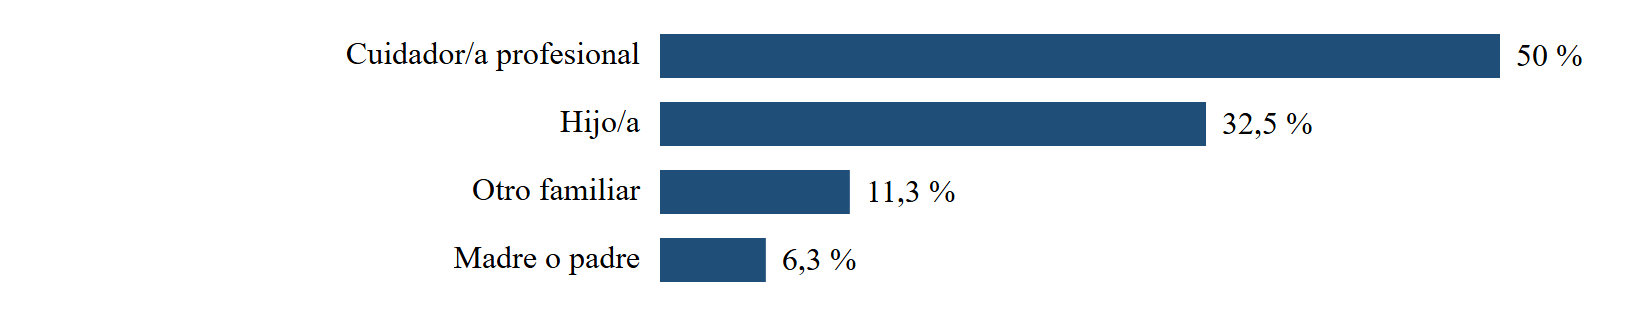
\includegraphics[width=\textwidth]{figuras/fig-7-1}
\caption{Relación con la persona que cuida (estudio simulado, 80 casos)}\label{fig:fig-7-1}
\end{figure}

{\small
\begin{xltabular}{\textwidth}{>{\raggedright\arraybackslash}X >{\raggedright\arraybackslash}X l}
\caption{Perfil de los casos del estudio simulado}\label{tab:c7-1}\\
\toprule
\tb{Pregunta} & \tb{Respuesta} & \tb{Casos} \\
\midrule
\endfirsthead
\toprule
\tb{Pregunta} & \tb{Respuesta} & \tb{Casos} \\
\midrule
\endhead
\bottomrule
\endfoot
Tiempo que lleva cuidando & Menos de 1 año & 17,5~\% \\
 & Entre 1 y 3 años & 57,5~\% \\
 & Entre 4 y 7 años & 3,8~\% \\
 & Más de 7 años & 21,3~\% \\
Horas por día dedicadas al cuidado & Menos de 4 horas & 25,0~\% \\
 & Entre 4 y 8 horas & 60,0~\% \\
 & Entre 8 y 12 horas & 7,5~\% \\
 & Más de 12 horas & 7,5~\% \\
Tipo de discapacidad de la persona & Motora & 32,5~\% \\
 & Intelectual & 27,5~\% \\
 & Autismo (TEA) & 20,0~\% \\
 & Visual & 15,0~\% \\
 & Múltiple & 5,0~\% \\
\end{xltabular}
}

\subsection{Organizar la información del cuidado}

Al 57,5~\% le resulta difícil o muy difícil organizar la información relacionada con el cuidado, como los turnos, la medicación, los estudios o los certificados. Solo al 2,5~\% le resulta fácil. El nivel de estrés que genera esa organización se ubica en un punto intermedio para la mayoría, con un promedio de 2,9 sobre 5, y el 76,3~\% lo califica como moderado.

\begin{figure}[H]
\centering
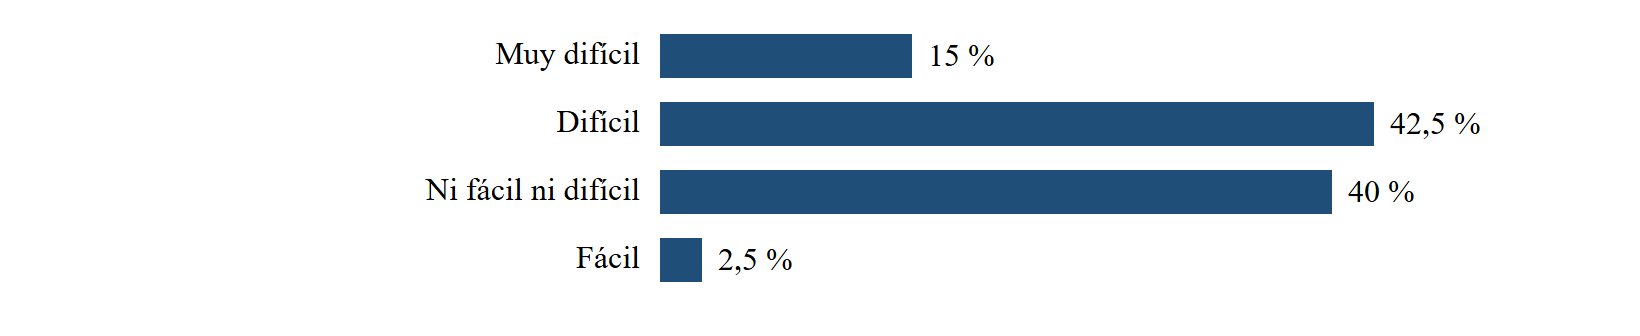
\includegraphics[width=\textwidth]{figuras/fig-7-2}
\caption{Dificultad para organizar la información del cuidado}\label{fig:fig-7-2}
\end{figure}

Entre los problemas más frecuentes se destaca sentirse acompañado o recibir orientación, que mencionan dos de cada tres casos. Le siguen coordinar tareas con otros cuidadores, controlar la medicación, encontrar información confiable y recordar los turnos médicos.

\begin{figure}[H]
\centering
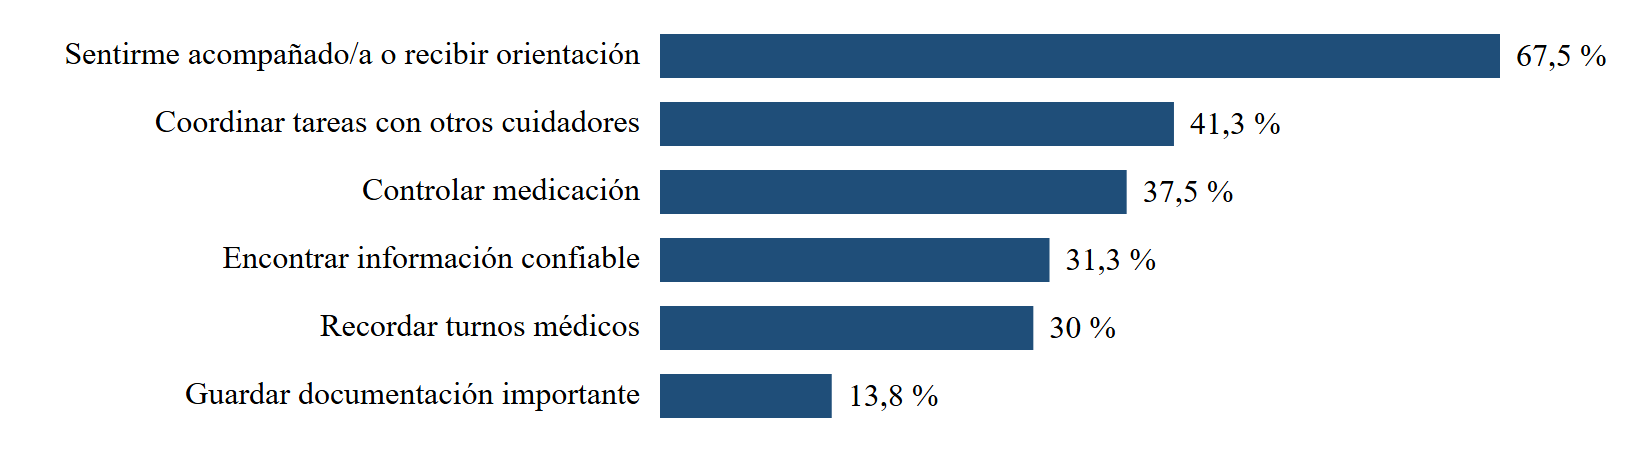
\includegraphics[width=\textwidth]{figuras/fig-7-3}
\caption{Problemas más frecuentes (respuesta múltiple)}\label{fig:fig-7-3}
\end{figure}

La dificultad para coordinar con otros cuidadores aparece sobre todo entre quienes cuidan de forma profesional. La señala el 62,5~\% de los cuidadores profesionales, frente al 20~\% de los familiares.

\subsection{Herramientas que se usan hoy}

La agenda en papel es la herramienta más usada, por el 87,5~\% de los casos, seguida por el calendario del celular, con un 62,5~\%, y por WhatsApp, con un 36,3~\%. El 71,3~\% combina dos herramientas o más, lo que muestra que la información del cuidado está repartida entre varios lugares. Solo el 2,5~\% no usa ninguna.

\begin{figure}[H]
\centering
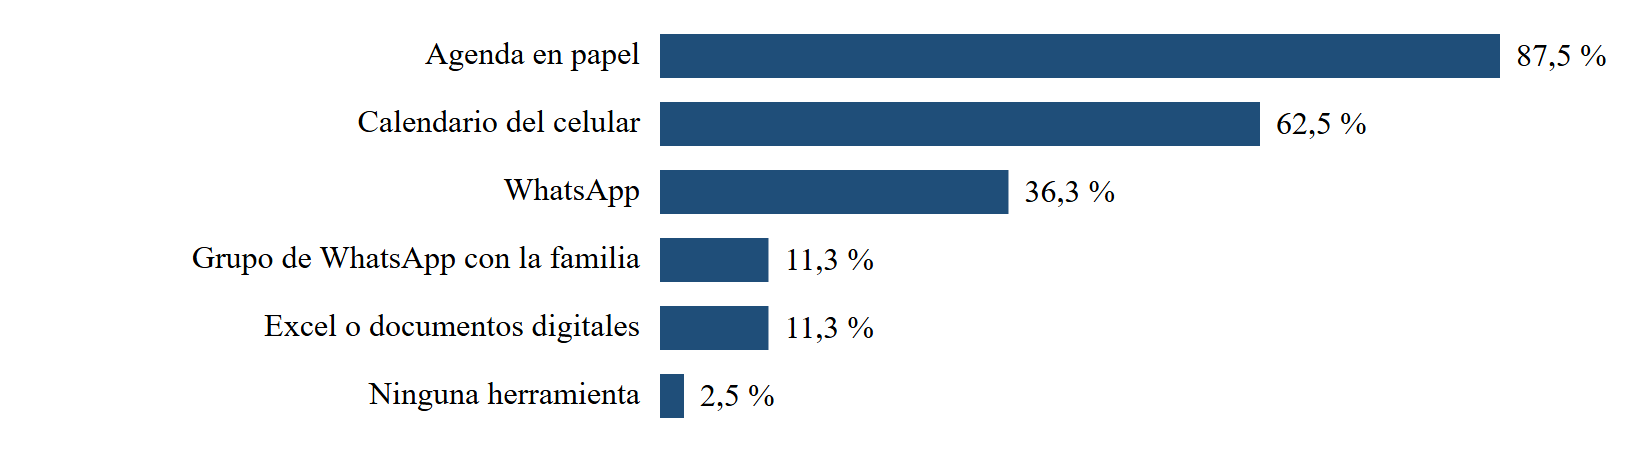
\includegraphics[width=\textwidth]{figuras/fig-7-4}
\caption{Herramientas que se usan hoy para organizar el cuidado (respuesta múltiple)}\label{fig:fig-7-4}
\end{figure}

\subsection{Interés en una herramienta como la propuesta}

El 80~\% considera que una herramienta como la propuesta le resultaría muy o bastante útil, y nadie respondió que no le serviría. El 61,3~\% afirma que usaría una aplicación web o móvil para gestionar el cuidado y el 38,8~\% no está seguro, mientras que ningún caso respondió que no la usaría. En la pregunta abierta, lo que más ayudaría hoy es tener resuelta la medicación y las rutinas, mejorar el acceso al sistema de salud, tener la información en un solo lugar y conseguir turnos con más facilidad.

\begin{figure}[H]
\centering
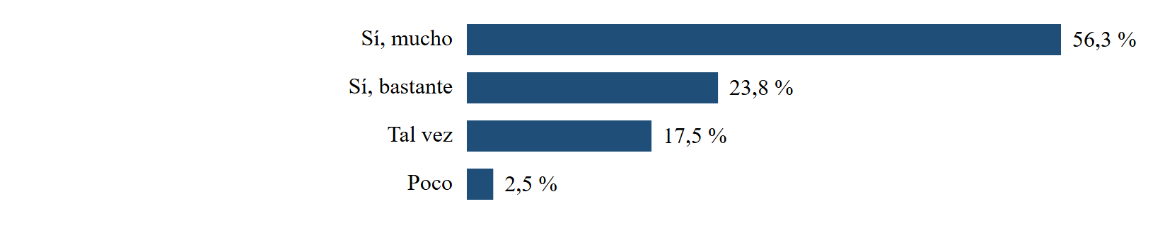
\includegraphics[width=\textwidth]{figuras/fig-7-5}
\caption{¿Una herramienta así le sería útil?}\label{fig:fig-7-5}
\end{figure}

\subsection{Qué decisiones de diseño se tomaron a partir del relevamiento}

\begin{table}[H]
\centering
\caption{Hallazgos del relevamiento y respuesta del sistema}\label{tab:c7-2}
\small
\begin{tabularx}{\textwidth}{>{\raggedright\arraybackslash}X >{\raggedright\arraybackslash}X}
\toprule
\tb{Hallazgo} & \tb{Cómo lo responde el sistema} \\
\midrule
La mitad de los casos son cuidadores profesionales y les cuesta coordinar con otros. & Grupos de cuidado con dueño, cuidadores y observadores, cada uno con su cuenta, y el registro de quién hizo cada cosa. \\
Dos de cada tres no se sienten acompañados ni orientados. & Guía de trámites, recursos y artículos según la discapacidad de la persona, y la sección Tu bienestar con líneas de ayuda. \\
La información está en la agenda de papel, el celular y WhatsApp. & Tu día reúne turnos y medicación en un solo lugar, con la ficha y los documentos de cada persona. \\
Controlar la medicación y recordar los turnos son problemas frecuentes. & Agenda de tomas con quién dio cada una, avisos de tomas atrasadas, recetas por vencer y controles que se repiten. \\
Encontrar información confiable cuesta. & Cada recurso y cada paso de la guía de trámites enlaza a su fuente oficial, y cada recomendación explica por qué aparece. \\
\bottomrule
\end{tabularx}
\end{table}

\section{Punto de partida}

Al comenzar esta etapa, el proyecto contaba con un prototipo de interfaz, una aplicación web autocontenida, sin servidor, con datos ficticios escritos directamente en el código y con un motor de recomendación que solo mostraba puntajes de ejemplo. Se habían fijado cuatro pasos siguientes. Implementar la API REST y el modelo de datos, migrar la interfaz a React con Vite, desarrollar una primera versión del motor de recomendación y validar la plataforma con usuarios.

Los tres primeros pasos se completaron. La plataforma pasó a ser un sistema funcional, con persistencia en base de datos, autenticación real, control de accesos por usuario y un motor de recomendación que calcula sus resultados a partir del perfil de cada persona asistida. Además, el motor incorporó la valoración de los cuidadores, con lo que pasó a funcionar como un sistema híbrido.

A partir de la revisión del sistema con el director del proyecto, el alcance se ajustó. Se retiraron la comunidad de cuidadores y el rol de especialista, y en su lugar se incorporó una sección de artículos ya publicados por especialistas, seleccionados y con enlace a su fuente. Se agregaron los grupos de cuidado, en los que el dueño de una cuenta ya sea una familia o una institución, suma cuidadores y observadores con su propia cuenta, y un modelo de tres planes con una base gratuita. Más adelante, los recursos y los artículos pasaron a mostrarse según el tipo de discapacidad de cada persona.

\section{Requisitos funcionales y estado de cumplimiento}

{\small
\begin{xltabular}{\textwidth}{l >{\raggedright\arraybackslash}X l >{\raggedright\arraybackslash}X}
\caption{Requisitos funcionales y estado de cumplimiento}\label{tab:rf}\\
\toprule
\tb{ID} & \tb{Requisito} & \tb{Estado} & \tb{Observaciones} \\
\midrule
\endfirsthead
\toprule
\tb{ID} & \tb{Requisito} & \tb{Estado} & \tb{Observaciones} \\
\midrule
\endhead
\bottomrule
\endfoot
RF01 & Registro, inicio de sesión y recuperación de contraseña por correo. & Cumplido & Un solo tipo de cuenta. Quien se registra es dueño de su grupo. \\
RF02 & Alta, edición y baja de personas asistidas con su perfil (tipo de discapacidad, obra social, localidad, necesidades). & Cumplido & El tipo de discapacidad es obligatorio, porque define recursos, artículos y estudios. \\
RF03 & Grupo de cuidado con cuidadores y observadores, cada uno con su cuenta. & Cumplido & El dueño suma integrantes con su correo y elige a qué personas acompaña cada uno. El cuidador registra y el observador solo mira. \\
RF04 & Seguimiento del grupo por persona y por cuidador. & Cumplido & Todo lo registrado con su autor, tomas sin registrar y, con el plan Plus, el cumplimiento de cada cuidador. \\
RF05 & Planes Básico, Intermedio y Plus con sus límites. & Parcial & Los límites se controlan en la API y en la interfaz. El pago está simulado, sin pasarela real. \\
RF06 & Agenda de turnos médicos con vista de calendario y controles que se repiten. & Cumplido & Vista mensual, próximos turnos y aviso un mes antes de cada control periódico. \\
RF07 & Registro de medicación con agenda diaria de tomas. & Cumplido & Se registra quién dio cada toma y se avisan recetas por vencer. \\
RF08 & Carga, búsqueda y descarga de documentos (estudios, recetas, certificados). & Cumplido & Con validación del tipo real de archivo y espacio según el plan. \\
RF09 & Módulo de emergencia con acceso al SAME (107) y a la red de apoyo. & Cumplido & Disponible en todos los planes. El llamado se resuelve con un enlace telefónico directo. \\
RF10 & Ficha de emergencia imprimible por persona. & Cumplido & Grupo sanguíneo, alergias, diagnóstico, médico y obra social. \\
RF11 & Guía de trámites según el tipo de discapacidad, con seguimiento del avance. & Cumplido & Basada en normativa oficial. Cada paso indica su fuente. \\
RF12 & Recursos específicos de la discapacidad de la persona, ordenados por relevancia y explicados. & Cumplido & Cada tarjeta muestra por qué se recomienda. \\
RF13 & Valoración de los recursos por parte del cuidador (``me sirvió'' / ``no me sirvió''). & Cumplido & Alimenta la parte colaborativa del recomendador. \\
RF14 & Artículos de especialistas por tipo de discapacidad y generales sobre el cuidado. & Cumplido & 20 artículos ya publicados, cada uno con su fuente y su enlace. \\
RF15 & Diario de cuidado con resumen imprimible para la consulta médica. & Cumplido & Incluye la medicación actual, las tomas que se dieron y las que no. \\
RF16 & Autoevaluación del esfuerzo del cuidador con orientación y líneas de ayuda. & Cumplido & Índice de Esfuerzo del Cuidador (13 preguntas). \\
RF17 & Administración de recursos y artículos. & Cumplido & Alta, edición y baja, con uno o más tipos de discapacidad por recurso. No se revisó en el navegador en esta instancia. \\
\end{xltabular}
}

De los 17 requisitos, 16 se cumplieron por completo y 1 de forma parcial.

La tabla~\ref{tab:rf-criterios} define la prioridad y el criterio de aceptación de cada requisito, y lo vincula con el indicador del capítulo~\ref{cap:metodologia} al que aporta.

{\small
\begin{xltabular}{\textwidth}{l l >{\raggedright\arraybackslash}X >{\raggedright\arraybackslash}p{3.2cm}}
\caption{Prioridad, criterio de aceptación e indicador de cada requisito funcional}\label{tab:rf-criterios}\\
\toprule
\tb{ID} & \tb{Prioridad} & \tb{Criterio de aceptación} & \tb{Indicador} \\
\midrule
\endfirsthead
\toprule
\tb{ID} & \tb{Prioridad} & \tb{Criterio de aceptación} & \tb{Indicador} \\
\midrule
\endhead
\bottomrule
\endfoot
RF01 & Alta & Una cuenta nueva se registra, inicia sesión y recupera la contraseña por correo sin intervención manual. & Facilidad de uso \\
RF02 & Alta & Una persona se crea, edita y borra, y al borrarla se eliminan todos sus registros. & Facilidad de uso \\
RF03 & Alta & Un observador recibe un error al intentar registrar y un cuidador solo ve a las personas que tiene asignadas. & Percepción de apoyo \\
RF04 & Media & El dueño ve el autor de cada registro y las tomas sin registrar de los últimos 7 días. & Percepción de apoyo \\
RF05 & Media & Una cuenta del plan Básico no puede crear una segunda persona ni abrir secciones de otros planes. & Intención de uso \\
RF06 & Alta & Un control que se repite genera un aviso 30 días antes del próximo turno. & Utilidad percibida \\
RF07 & Alta & Cada toma guarda quién la registró y a qué hora, y se avisa la receta próxima a vencer. & Utilidad percibida \\
RF08 & Media & Se rechaza un archivo cuyo contenido no coincide con su extensión y se respeta el espacio del plan. & Facilidad de uso \\
RF09 & Alta & El acceso al 107 está visible en todas las pantallas y en todos los planes. & Percepción de apoyo \\
RF10 & Media & La ficha impresa incluye grupo sanguíneo, alergias, diagnóstico, médico y obra social. & Utilidad percibida \\
RF11 & Alta & Cada paso de la guía muestra su fuente oficial y el avance se guarda por persona. & Utilidad percibida \\
RF12 & Alta & El 100~\% de las recomendaciones tiene explicación y todas son del tipo de discapacidad de la persona. & Recomendaciones explicadas \\
RF13 & Media & Una valoración cambia el orden de las recomendaciones de personas con la misma discapacidad. & Precisión del recomendador \\
RF14 & Media & Cada artículo tiene fuente y enlace verificado, con al menos uno por tipo de discapacidad. & Cobertura del catálogo \\
RF15 & Media & El resumen imprimible incluye la medicación actual y las tomas dadas y no dadas. & Utilidad percibida \\
RF16 & Baja & El cuestionario de 13 preguntas calcula el resultado y muestra orientación y líneas de ayuda. & Percepción de apoyo \\
RF17 & Baja & Una cuenta de administración crea, edita y desactiva recursos y artículos. & Cobertura del catálogo \\
\end{xltabular}
}

\section{Requisitos no funcionales y evidencia obtenida}

\begin{table}[H]
\centering
\caption{Requisitos no funcionales y evidencia obtenida}\label{tab:rnf}
\footnotesize
\begin{tabularx}{\textwidth}{l >{\raggedright\arraybackslash}X >{\raggedright\arraybackslash}X >{\raggedright\arraybackslash}X}
\toprule
\tb{ID} & \tb{Requisito} & \tb{Evidencia} & \tb{Estado} \\
\midrule
RNF01 & Usabilidad y accesibilidad & Tipografía de alta legibilidad, tres tamaños de letra, modo de alto contraste, foco visible al navegar con teclado y textos en lenguaje claro. & Cumplido a nivel técnico, falta validar con usuarios \\
RNF02 & Diseño adaptable a celulares & Las doce pantallas se revisaron a 375 px de ancho, sin desplazamiento horizontal. En celulares la navegación pasa a una barra inferior. & Cumplido \\
RNF03 & Seguridad de acceso & Contraseñas con hash, token firmado, roles, bloqueo de la cuenta durante 5 minutos tras 5 intentos fallidos y filtrado de los datos por persona asistida. & Cumplido \\
RNF04 & Privacidad entre grupos & Cada usuario ve solo sus personas y las de los grupos donde ayuda. Cada cuidador ve solo a quienes tiene asignados y nadie ve el grupo de otro dueño, cubierto por pruebas automatizadas. & Cumplido \\
RNF05 & Tiempo de respuesta & Mediana de 6,8 ms y percentil 95 de 9,2 ms al calcular recomendaciones. & Cumplido (medido en el entorno local) \\
RNF06 & Mantenibilidad & 18 migraciones versionadas del esquema, 68 pruebas automatizadas, separación en capas y código en un repositorio con control de versiones. & Cumplido \\
RNF07 & Disponibilidad en la nube & Todavía no se publicó. El sistema se ejecuta en un entorno local y la publicación en Azure App Service y Azure SQL Database queda como próximo paso. & Pendiente \\
\bottomrule
\end{tabularx}
\end{table}

\begin{table}[H]
\centering
\caption{Prioridad y criterio de aceptación de cada requisito no funcional}\label{tab:rnf-criterios}
\small
\begin{tabularx}{\textwidth}{l l >{\raggedright\arraybackslash}X}
\toprule
\tb{ID} & \tb{Prioridad} & \tb{Criterio de aceptación} \\
\midrule
RNF01 & Alta & Todas las pantallas se recorren con teclado y el texto admite tres tamaños sin perder información. \\
RNF02 & Alta & Ninguna pantalla genera desplazamiento horizontal a 375 px de ancho. \\
RNF03 & Alta & Las contraseñas se guardan con hash y la cuenta se bloquea tras 5 intentos fallidos. \\
RNF04 & Alta & Ninguna prueba automatizada de acceso entre grupos permite ver o modificar datos ajenos. \\
RNF05 & Media & El cálculo de recomendaciones responde en menos de 1 segundo en el percentil 95. \\
RNF06 & Media & El esquema se reproduce con las migraciones y las pruebas se ejecutan con un solo comando. \\
RNF07 & Media & El sistema es accesible públicamente por HTTPS. \\
\bottomrule
\end{tabularx}
\end{table}

\section{Arquitectura implementada}

Se respetó la arquitectura en capas descripta en el Capítulo 4, una interfaz web en React, una API REST en ASP.NET Core que contiene la lógica de negocio y el motor de recomendación, y una base de datos relacional en SQL Server.

\begin{table}[H]
\centering
\caption{Diferencias entre la arquitectura planificada y la implementada}\label{tab:c7-5}
\footnotesize
\begin{tabularx}{\textwidth}{>{\raggedright\arraybackslash}X >{\raggedright\arraybackslash}X >{\raggedright\arraybackslash}X}
\toprule
\tb{Aspecto} & \tb{Planificado} & \tb{Implementado y motivo} \\
\midrule
Control de acceso a los datos & Row-Level Security de SQL Server. & Un único servicio de la API decide, para cada persona asistida, si el usuario puede verla, registrar en ella o administrarla, y todos los controladores lo usan. Se eligió así para poder probarlo con pruebas automatizadas. \\
Cifrado en reposo & Transparent Data Encryption en Azure SQL. & Pendiente. Se activará al publicar en Azure SQL Database, que aplica Transparent Data Encryption por defecto. Hoy se usa SQL Server Express en el entorno local, solo con datos de demostración. \\
Conexión con el SAME & API de emergencias del SAME. & Enlace telefónico directo al 107 visible desde todas las pantallas. No existe una API pública, como se previó en el riesgo R7. \\
Motor de recomendación & Basado en contenido en la primera versión. & Híbrido. Perfil de la persona más valoraciones de los cuidadores. \\
Cobro de los planes & Pasarela de pagos. & Cambio de plan simulado desde la cuenta. Los límites de cada plan sí se aplican en la API. \\
Sesión del usuario & Token emitido por la API. & Token JWT guardado en el navegador. Es aceptable para un prototipo, pero una cookie protegida reduciría el riesgo ante ataques de inyección de código. \\
Cuentas & Cuentas de familia y de institución por separado. & Un solo tipo de cuenta. Una institución es el dueño de un grupo con plan Plus, lo que simplifica el modelo y sirve igual para una familia grande. \\
\bottomrule
\end{tabularx}
\end{table}

\section{Modelo de datos}

El modelo de datos quedó compuesto por 14 entidades propias, además de las tablas de usuarios y roles que provee ASP.NET Core Identity. Pueden agruparse en cinco bloques. La persona asistida y su cuidado diario (turnos, medicamentos, tomas, diario y documentos), la emergencia (contactos y ficha, incluida en la persona), la orientación (recursos, valoraciones de recursos, avance de trámites y artículos), la organización del cuidado (los integrantes de cada grupo) y el bienestar del cuidador (evaluaciones de esfuerzo).

Cada persona asistida tiene un responsable, que es el dueño del grupo. Los integrantes se resuelven con una tabla que vincula a la persona con cada usuario y su rol, cuidador u observador, sin modificar quién es el dueño. El plan y el nombre del grupo se guardan en la cuenta del dueño, y el plan que cubre a cada persona es siempre el de su dueño.

Las relaciones se definieron con claves foráneas y, en los casos que corresponde, con borrado en cascada. Al eliminar una persona asistida se eliminan sus turnos, medicamentos, documentos, valoraciones, avances de trámites e integrantes del grupo. Para evitar registros duplicados se agregaron índices únicos, por ejemplo, una sola valoración por persona y recurso, y una sola toma por medicamento, día y horario.

\section{Diseño de la interfaz}

El diseño de la interfaz siguió los principios de la norma ISO 9241-210 \citep{une2019}. Se adoptó la tipografía Atkinson Hyperlegible, desarrollada por el Braille Institute para personas con baja visión, y se limitó el uso del color a lo que transmite información, un color de acento para lo que requiere atención, rojo solo para la emergencia y un color distinto por cada persona asistida, de modo que en el calendario o en la medicación se reconozca a quién corresponde cada registro.

La pantalla de inicio se organizó como una línea del día, que reúne en orden horario los turnos y las tomas de medicación y permite registrar una toma sin cambiar de sección. El menú agrupa las secciones según para qué se usan. Cuidado diario reúne lo que se registra de cada persona, Orientación lo que se consulta para saber qué hacer, Quienes cuidan el grupo y el bienestar de quien cuida, y Cuenta el plan. La interfaz se adapta a lo que cada persona puede hacer. A un observador no se le muestran los botones para registrar, a la dueña de una residencia se le muestra el estado de cada toma y a cargo de quién está, y lo que no incluye el plan aparece con una explicación de qué plan lo incluye.

\section{Construcción e integración}

El código fuente completo está disponible en el repositorio descripto en el anexo~\ref{anx:repositorios}, y el apéndice~B explica cómo ejecutarlo en un entorno local. Su publicación en Azure queda como próximo paso.

El desarrollo se realizó de forma incremental. Cada módulo se construyó primero en la API, con su entidad y su migración, luego se integró en la interfaz y por último se probó de punta a punta.

\begin{table}[H]
\centering
\caption{Dimensiones del sistema construido}\label{tab:c7-6}
\small
\begin{tabularx}{\textwidth}{>{\raggedright\arraybackslash}X >{\raggedright\arraybackslash}X}
\toprule
\tb{Indicador} & \tb{Valor} \\
\midrule
Endpoints de la API & 68, distribuidos en 14 controladores \\
Entidades del modelo de datos & 14 (más las de Identity) \\
Migraciones del esquema & 18 \\
Vistas de la interfaz & 13 \\
Líneas de código del backend (sin migraciones) & 7.358 \\
Líneas de código del frontend (JavaScript y JSX) & 7.946 \\
Líneas de hojas de estilo & 5.528 \\
Líneas de código de pruebas automatizadas & 896 \\
\bottomrule
\end{tabularx}
\end{table}

Para probar el sistema en condiciones parecidas a las reales se cargó un conjunto de datos de demostración. Ocho familias con distintos planes y nueve personas asistidas de distintos tipos de discapacidad, obras sociales y localidades, una cuidadora contratada que atiende a personas de dos familias, una familiar en modo observador, y una residencia con su dueña, dos cuidadores y cuatro residentes. Al iniciar, el sistema completa la última semana de tomas y corre el diario de prueba, para que la demostración refleje siempre días recientes. Todos los datos son ficticios. El código se guarda en un repositorio privado con control de versiones.

\section{Motor de recomendación}

El motor se implementó como un servicio interno de la API, sin librerías externas de aprendizaje automático. Cada recurso del catálogo corresponde a uno o más tipos de discapacidad, y el motor solo considera los del tipo de la persona. Lo que sirve a cualquier persona, como el CUD, la pensión o el transporte, está en la guía de trámites. Para cada recurso del tipo de la persona sigue tres pasos. Primero descarta los que piden algo que la persona no cumple, un recurso de PAMI no se muestra a quien tiene otra obra social, ni uno de Rosario a alguien de Escobar, y uno marcado como ``sin obra social'' no se muestra a quien tiene una. Después suma puntos por cada coincidencia entre el perfil y el recurso. Por último, ajusta el orden según las valoraciones.

\begin{table}[H]
\centering
\caption{Pesos utilizados por el motor de recomendación}\label{tab:c7-7}
\small
\begin{tabularx}{\textwidth}{>{\raggedright\arraybackslash}X l >{\raggedright\arraybackslash}X}
\toprule
\tb{Criterio} & \tb{Puntos} & \tb{Cuándo se aplica} \\
\midrule
Tipo de discapacidad & 40 & El recurso es para el tipo de discapacidad de la persona. Es condición para que aparezca. \\
Necesidades & 35 & El recurso responde a al menos una de las necesidades marcadas en el perfil. \\
Obra social & 30 & El recurso es de la obra social de la persona. \\
Localidad & 30 & El recurso está en la localidad de la persona. \\
Valoración propia positiva & +30 & Quien cuida a la persona marcó ``me sirvió''. \\
Valoración propia negativa & al final & Quien cuida marcó ``no me sirvió''. El recurso pasa al final de la lista, sin desaparecer. \\
Valoraciones de otros cuidadores & hasta $\pm$20 & Votos de cuidadores de personas con el mismo tipo de discapacidad. Con menos de tres votos el ajuste se reduce en proporción. \\
\bottomrule
\end{tabularx}
\end{table}

El porcentaje de coincidencia que ve el usuario se calcula solo con los puntos del perfil, sobre un máximo de 135. Las valoraciones modifican el orden, pero no ese porcentaje, para que el número siga expresando cuánto se ajusta el recurso a la situación de la persona. Cada criterio que suma puntos genera una explicación, y cuando un recurso sube por las valoraciones de otros se indica a cuántos cuidadores les sirvió.

La parte colaborativa compara solamente con personas del mismo tipo de discapacidad, de modo que una valoración sobre un recurso para personas con discapacidad motora no influye en lo que se le muestra a una familia que cuida a alguien con discapacidad visual. Con esto se atiende el problema del arranque en frío descripto en el Capítulo 3, ya que mientras no haya valoraciones el sistema funciona igual que uno basado en contenido.

\section{Contenido de orientación}\label{sec:contenido}

La guía de trámites se armó a partir de las normativas oficiales de certificación de la discapacidad (Disposiciones del Servicio Nacional de Rehabilitación 1019, 639, 82, 648 y 500 de 2015) y de páginas oficiales de argentina.gob.ar, la Superintendencia de Servicios de Salud, la CNRT y ANSES. Se organiza en cuatro etapas. La consulta de requisitos del CUD, los estudios que corresponden según el tipo de discapacidad, la presentación ante la junta evaluadora y los derechos a los que se accede con el certificado. Cada paso indica su fuente y su enlace, y una prueba automatizada verifica que ninguno quede sin fuente.

El catálogo de recursos recomendables quedó integrado por 20 recursos activos, todos de uno o más tipos de discapacidad. Diez son de alcance nacional y diez son locales, ubicados en Pilar, la Ciudad de Buenos Aires, Córdoba, La Plata, Rosario, Escobar, Tigre y San Isidro. La sección de artículos reúne 20 textos ya publicados, seis generales sobre el cuidado y catorce de un tipo de discapacidad, de modo que cada tipo tiene al menos uno. Provienen de materiales oficiales para cuidadores, de la Organización Mundial de la Salud y la Organización Panamericana de la Salud, y de revistas científicas, y cada uno lleva a su fuente original.

\section{Pruebas automatizadas}

Se desarrolló un proyecto de pruebas con xUnit que utiliza una base de datos SQLite en memoria, de manera que cada prueba trabaja sobre datos propios y no depende de la base real. Las pruebas se concentraron en las partes donde un error tendría consecuencias más graves, el acceso a datos de terceros, los permisos dentro de los grupos, los límites de los planes, el cálculo de las recomendaciones, la guía de trámites y la escala de esfuerzo.

\begin{table}[H]
\centering
\caption{Pruebas automatizadas por área}\label{tab:c7-8}
\footnotesize
\begin{tabularx}{\textwidth}{>{\raggedright\arraybackslash}X >{\raggedright\arraybackslash}X l l}
\toprule
\tb{Clase de prueba} & \tb{Qué verifica} & \tb{Casos} & \tb{Ok} \\
\midrule
AccesoCompartidoTests & Que cada usuario vea solo sus personas y las de su grupo, que alguien ajeno no pueda modificar la medicación y que al borrar una persona se borre todo lo suyo. & 8 & 8 \\
EquipoYPlanesTests & Que el observador vea sin registrar, que el cuidador registre sin administrar, que cada cuidador vea solo a sus asignados y quede cubierto por el plan del dueño, que nadie vea el grupo de otro, lo que el dueño ve de cada uno y los límites de cada plan. & 16 & 16 \\
RecomendacionServiceTests & El orden por coincidencia, que solo aparezcan recursos del tipo de la persona, el descarte por localidad y por ``sin obra social'', la tolerancia a mayúsculas y tildes, el tope del porcentaje y el efecto de las valoraciones. & 10 & 10 \\
GuiaTramitesTests & Que cada tipo de discapacidad vea solo sus estudios, los pasos según la edad y el parentesco, y que todos los pasos tengan fuente y enlace oficial. & 15 & 15 \\
EscalaEsfuerzoTests & Las 13 preguntas del índice, el punto de corte en 7 respuestas afirmativas y las sugerencias derivadas. & 5 & 5 \\
FormatoTests & Horarios de medicación válidos e inválidos, el nombre que se muestra sin título profesional y la regla de las cuentas de demostración. & 14 & 14 \\
\textbf{Total} &  & \textbf{68} & \textbf{68} \\
\bottomrule
\end{tabularx}
\end{table}

Las 68 pruebas se ejecutaron con resultado satisfactorio. Además, la compilación del backend no registra advertencias y el análisis estático del frontend no informa errores.

\section{Pruebas de integración}

Las pruebas de integración se realizaron contra la API en ejecución y desde el navegador, recorriendo los flujos completos. Registro e inicio de sesión, alta y edición de una persona, cálculo de recomendaciones, carga de turnos, subida de un documento válido y rechazo de un archivo con extensión falsa, descarga, registro de tomas y valoración de recursos. Para los grupos se verificó sumar a una observadora y quitarla, cambiar a quiénes acompaña un cuidador, que un observador reciba un error de permiso al intentar registrar una toma y que cada plan habilite solo lo que le corresponde. También se probó el aviso de un control que se repite con un turno de prueba. Los datos creados para estas pruebas se eliminaron al finalizar.

\section{Pruebas de interfaz y accesibilidad}\label{sec:interfaz}

La interfaz se revisó en pantallas de computadora y a 375 px de ancho, equivalente a un celular, con cuentas de distintos roles, la dueña de una residencia, una familia con cada uno de los tres planes, una cuidadora contratada y una observadora. Se comprobó que cada rol vea solo las acciones que le corresponden y que ninguna de las doce pantallas genere desplazamiento horizontal. También se revisaron la combinación de letra muy grande con alto contraste y la navegación con teclado.

\section{Rendimiento}

Se midió el tiempo de respuesta del cálculo de recomendaciones, que es la operación más costosa del sistema porque recorre el catálogo y las valoraciones. Se tomaron 65 mediciones, cinco por cada una de las trece personas evaluadas, en el equipo de desarrollo y descartando la primera llamada de cada persona.

\begin{table}[H]
\centering
\caption{Tiempo de respuesta del cálculo de recomendaciones}\label{tab:c7-9}
\small
\begin{tabularx}{\textwidth}{l l}
\toprule
\tb{Medida} & \tb{Valor} \\
\midrule
Mediciones & 65 \\
Promedio & 7,1 ms \\
Mediana & 6,8 ms \\
Percentil 95 & 9,2 ms \\
Máximo & 9,9 ms \\
\bottomrule
\end{tabularx}
\end{table}

Los tiempos son bajos para el volumen actual, pero se midieron en el entorno local de desarrollo, con un catálogo de 20 recursos. No permiten anticipar el comportamiento con miles de recursos ni con muchos usuarios simultáneos una vez publicado en Azure.

\section{Seguimiento del grupo con los datos de demostración}\label{sec:seguimiento}

Para comprobar que el panel del grupo permite detectar diferencias en el trabajo de cada cuidador, se usaron los registros de la última semana de la residencia de demostración. Una cuidadora registra todas las tomas a tiempo y el otro deja tomas sin registrar y anota tarde. El panel mostró los resultados que se esperaban a partir de esos datos.

\begin{table}[H]
\centering
\caption{Indicadores del panel del grupo (últimos 7 días)}\label{tab:c7-10}
\small
\begin{tabularx}{\textwidth}{l >{\raggedright\arraybackslash}X l >{\raggedright\arraybackslash}X >{\raggedright\arraybackslash}X}
\toprule
\tb{Cuidador} & \tb{Tomas registradas} & \tb{Sin registrar} & \tb{Registradas tarde} & \tb{Entradas del diario} \\
\midrule
Carla Ruiz & 100~\% (39 de 39) & 0 & 0 & 3 \\
Diego Paredes & 70~\% (28 de 40) & 12 & 28 & 1 \\
\bottomrule
\end{tabularx}
\end{table}

Este resultado solo muestra que el panel calcula y presenta correctamente los indicadores. Si le resulta útil a una institución real, y si los indicadores se interpretan de manera adecuada, deberá evaluarse con instituciones, como se advierte en el riesgo R11.

\section{Defectos encontrados}

Durante las pruebas se registraron los siguientes defectos. Todos se corrigieron.

{\small
\begin{xltabular}{\textwidth}{l >{\raggedright\arraybackslash}X >{\raggedright\arraybackslash}X l}
\caption{Defectos detectados durante las pruebas}\label{tab:c7-11}\\
\toprule
\tb{ID} & \tb{Defecto} & \tb{Cómo se detectó} & \tb{Estado} \\
\midrule
\endfirsthead
\toprule
\tb{ID} & \tb{Defecto} & \tb{Cómo se detectó} & \tb{Estado} \\
\midrule
\endhead
\bottomrule
\endfoot
D1 & En celulares, el calendario mensual excedía el ancho de la pantalla (486 px de contenido en 375 px). & Revisión de interfaz en 375 px & Corregido \\
D2 & El menú ``Más'' del celular no se cerraba con la tecla Escape ni llevaba el foco al menú. & Prueba con teclado & Corregido \\
D3 & En pantallas angostas, los contactos de emergencia propios quedaban debajo de los números generales, fuera de la vista. & Observación de uso & Corregido \\
D4 & Cuatro recursos enlazaban a páginas inexistentes (error 404). & Revisión de enlaces & Corregido \\
D5 & Trece recursos enlazaban a portadas genéricas en lugar de la página del tema descripto. & Revisión de enlaces & Corregido \\
D6 & Tres recursos estaban duplicados por una versión anterior de los datos iniciales. & Revisión de la base de datos & Corregido \\
D7 & En celulares, el encabezado de la ficha de una persona excedía el ancho de la pantalla. & Revisión de interfaz en ancho de celular & Corregido \\
D8 & Una fila de filtros no pasaba a una segunda línea en pantallas angostas. & Revisión de interfaz en ancho de celular & Corregido \\
D9 & En la pantalla de planes, el precio del plan Básico aparecía repetido. & Revisión de interfaz & Corregido \\
D10 & El programa Incluir Salud se recomienda a personas afiliadas a PAMI, aunque solo corresponde a titulares de pensiones no contributivas sin obra social. & Evaluación del recomendador & Corregido \\
D11 & Algunos perfiles no reciben ningún recurso local ni específico de su discapacidad. & Evaluación del recomendador & Corregido \\
D12 & La sección Tu bienestar sugería ir a la comunidad de cuidadores, que ya no existía. & Revisión de contenido & Corregido \\
D13 & La página de ANSES de la pensión no contributiva no respondía. Se reemplazó por la página oficial de argentina.gob.ar. & Revisión de enlaces & Corregido \\
D14 & El aviso de controles que se repiten no aparecía porque la fecha del próximo control se calculaba mal. & Prueba con un turno de prueba & Corregido \\
\end{xltabular}
}

El defecto D10 se resolvió agregando al motor la condición ``sin obra social'', que deja un recurso solo para quien no tiene obra social o se atiende por Incluir Salud. El D11 se resolvió ampliando el catálogo con recursos reales en Escobar, Tigre y San Isidro y con recursos específicos para discapacidad visceral, visual y múltiple.

\section{Evaluación del motor de recomendación}\label{sec:eval-motor}

Para evaluar el motor se calcularon las recomendaciones de las trece personas asistidas de demostración, sobre el catálogo de 20 recursos. La tabla muestra, para cada perfil, cuántos recursos se recomendaron, cuántos eran locales y cuál quedó en primer lugar.

{\footnotesize
\begin{xltabular}{\textwidth}{l l l l l l >{\raggedright\arraybackslash}X}
\caption{Recomendaciones calculadas por perfil}\label{tab:c7-12}\\
\toprule
\tb{Persona} & \tb{Tipo} & \tb{Obra social} & \tb{Localidad} & \tb{Rec.} & \tb{Locales} & \tb{Primer recurso (coincidencia)} \\
\midrule
\endfirsthead
\toprule
\tb{Persona} & \tb{Tipo} & \tb{Obra social} & \tb{Localidad} & \tb{Rec.} & \tb{Locales} & \tb{Primer recurso (coincidencia)} \\
\midrule
\endhead
\bottomrule
\endfoot
Rosa F. & Motora & PAMI & Pilar & 6 & 2 & Centro de Rehabilitación Pilares de Esperanza (78~\%) \\
Tomás L. & Intelectual & IOMA & La Plata & 3 & 1 & Dirección de Educación Especial bonaerense (78~\%) \\
Héctor B. & Visual & PAMI & CABA & 2 & 1 & Baja visión en el Hospital Santa Lucía (52~\%) \\
Lucía R. & Auditiva & OSDE & Córdoba & 2 & 1 & Curso de Lengua de Señas en Córdoba (52~\%) \\
Martín S. & Psicosocial & Incluir Salud & Rosario & 2 & 1 & Atención en salud mental (56~\%) \\
Elena G. & Múltiple & PAMI & Escobar & 5 & 1 & Asistencia a personas con discapacidad en PAMI (78~\%) \\
Raúl G. & Motora & PAMI & Escobar & 5 & 1 & Símbolo Internacional de Acceso (56~\%) \\
Micaela P. & Motora & OSECAC & Tigre & 5 & 2 & Centro de Rehabilitación Frida Kahlo (78~\%) \\
Osvaldo V. & Visceral & PAMI & San Isidro & 2 & 1 & Derechos de las personas trasplantadas (56~\%) \\
Alberto N. & Motora & PAMI & Pilar & 6 & 2 & Asistencia a personas con discapacidad en PAMI (52~\%) \\
Ernesto V. & Visceral & PAMI & Pilar & 1 & 0 & Derechos de las personas trasplantadas (30~\%) \\
Norma C. & Visual & PAMI & Pilar & 1 & 0 & Biblioteca Argentina para Ciegos (30~\%) \\
Susana O. & Psicosocial & IOMA & Pilar & 1 & 0 & Atención en salud mental (30~\%) \\
\end{xltabular}
}

Las 41 recomendaciones generadas incluyeron una explicación (100~\%) y los 20 recursos del catálogo aparecieron en la lista de al menos un perfil. Todas las personas de las familias de demostración reciben ahora al menos un recurso local y uno específico de su tipo de discapacidad, con lo que se corrigió el defecto D11. Como cada recurso es de un tipo, las listas son más cortas que en la versión anterior, de entre uno y seis recursos, pero todos corresponden a la situación de la persona.

Los resultados también muestran el límite que se mantiene. Los residentes de Pilar con discapacidad visual, visceral o psicosocial reciben un solo recurso, de alcance nacional, porque el catálogo no tiene recursos locales de esos tipos en Pilar. La calidad de las recomendaciones depende del tamaño y del mantenimiento del catálogo, como se planteó como barrera en el Capítulo 1.

\section{Verificación de las fuentes de información}\label{sec:fuentes}

Dado que el riesgo R2 del Capítulo 6 advertía que la información sobre recursos podía estar dispersa o desactualizada, se revisaron uno por uno los enlaces de todo el sistema. Los 20 recursos, los 20 artículos, los pasos de la guía de trámites y las líneas de ayuda, en total 52 enlaces. El criterio fue que cada enlace llevara a la página que trata el tema descripto en la tarjeta, y que el texto de la tarjeta no prometiera algo que la página no dice.

En los recursos, el resultado inicial fue desfavorable, ya que ninguno de los 18 enlaces cumplía el criterio. Cuatro llevaban a páginas inexistentes, trece a portadas generales de organismos y uno a una página general en lugar del trámite. Además, los ocho recursos locales eran ficticios. Todos se reemplazaron por páginas oficiales específicas, se ajustaron las descripciones a lo que cada página informa y los recursos locales pasaron a ser instituciones y servicios reales. Los artículos se seleccionaron ya con este criterio, y sus 15 enlaces llevan al texto publicado.

Los recursos y artículos que se sumaron después se seleccionaron ya con este criterio, y en la última revisión todos los enlaces respondieron. El único que falló, la página de ANSES sobre la pensión no contributiva se reemplazó por la página oficial del trámite en argentina.gob.ar. También se confirmaron los teléfonos de las líneas de ayuda de Tu bienestar.

Se priorizaron fuentes de organismos nacionales, provinciales y municipales, y revistas científicas. Aun así, algunas pierden vigencia con el tiempo, por ejemplo, el curso de Lengua de Señas de Córdoba corresponde al ciclo 2026. Por eso existe la pantalla de administración, desde la que pueden corregirse o desactivarse recursos y artículos sin modificar el código.

\section{Cumplimiento de los objetivos específicos}\label{sec:objetivos-cumplidos}

\begin{table}[H]
\centering
\caption{Cumplimiento de los objetivos específicos}\label{tab:objetivos}
\footnotesize
\begin{tabularx}{\textwidth}{>{\raggedright\arraybackslash}X >{\raggedright\arraybackslash}X >{\raggedright\arraybackslash}X}
\toprule
\tb{Objetivo específico (Capítulo 1)} & \tb{Resultado} & \tb{Estado} \\
\midrule
Desarrollar un sistema de recomendación que combine el perfil de la persona con las valoraciones de otros cuidadores. & Motor híbrido que recomienda solo recursos del tipo de discapacidad de la persona, probado con pruebas automatizadas. Cada recomendación se explica. & Cumplido \\
Permitir que el cuidado se organice en grupos y que el dueño, familia o institución, siga el trabajo de cada cuidador. & Grupos con dueño, cuidadores y observadores, seguimiento por persona y por cuidador, y cumplimiento de cada cuidador con el plan Plus. & Cumplido \\
Incorporar un módulo de emergencia con contacto directo al SAME y a una red de apoyo. & Acceso al 107 desde todas las pantallas, contactos propios con llamada directa y ficha de emergencia imprimible, en todos los planes. & Cumplido \\
Diseñar una interfaz accesible e intuitiva, también para celulares. & Diseño adaptable revisado a 375 px, letra ampliable, alto contraste, navegación con teclado y acciones según el rol. & Cumplido a nivel técnico, pendiente de validación con usuarios \\
Guiar los trámites que corresponden según el tipo de discapacidad. & Guía en cuatro etapas con seguimiento del avance, basada en normativa oficial, con fuente en cada paso. & Cumplido \\
Reunir artículos de especialistas organizados por tipo de discapacidad. & 20 artículos publicados, con al menos uno por tipo de discapacidad, y su fuente y su enlace verificados. & Cumplido \\
\bottomrule
\end{tabularx}
\end{table}

\section{Síntesis de los resultados}

El resultado principal es que la propuesta pasó de un prototipo de interfaz a un sistema funcional que reúne en un solo lugar la organización del cuidado diario, la coordinación del grupo que cuida, la orientación sobre trámites, recursos y artículos según la discapacidad de cada persona, y la emergencia. El relevamiento analizado, mostró que la información del cuidado está repartida en varios lugares, que a más de la mitad le cuesta organizarla y que la falta de orientación es el problema más frecuente, y cada uno de esos hallazgos tiene una respuesta concreta en el sistema. Dieciséis de los diecisiete requisitos funcionales se cumplieron por completo, las 68 pruebas automatizadas resultaron satisfactorias, todos los defectos detectados se corrigieron y el motor de recomendación explica cada una de sus sugerencias, lo que responde a la barrera de credibilidad planteada al inicio del trabajo.

